La méthode de développement de projets informatique utilisée chez la \df est la méthode \gls{scrum}, une des implémentations du \gls{agile}.

\begin{figure}[H]
    \centering
    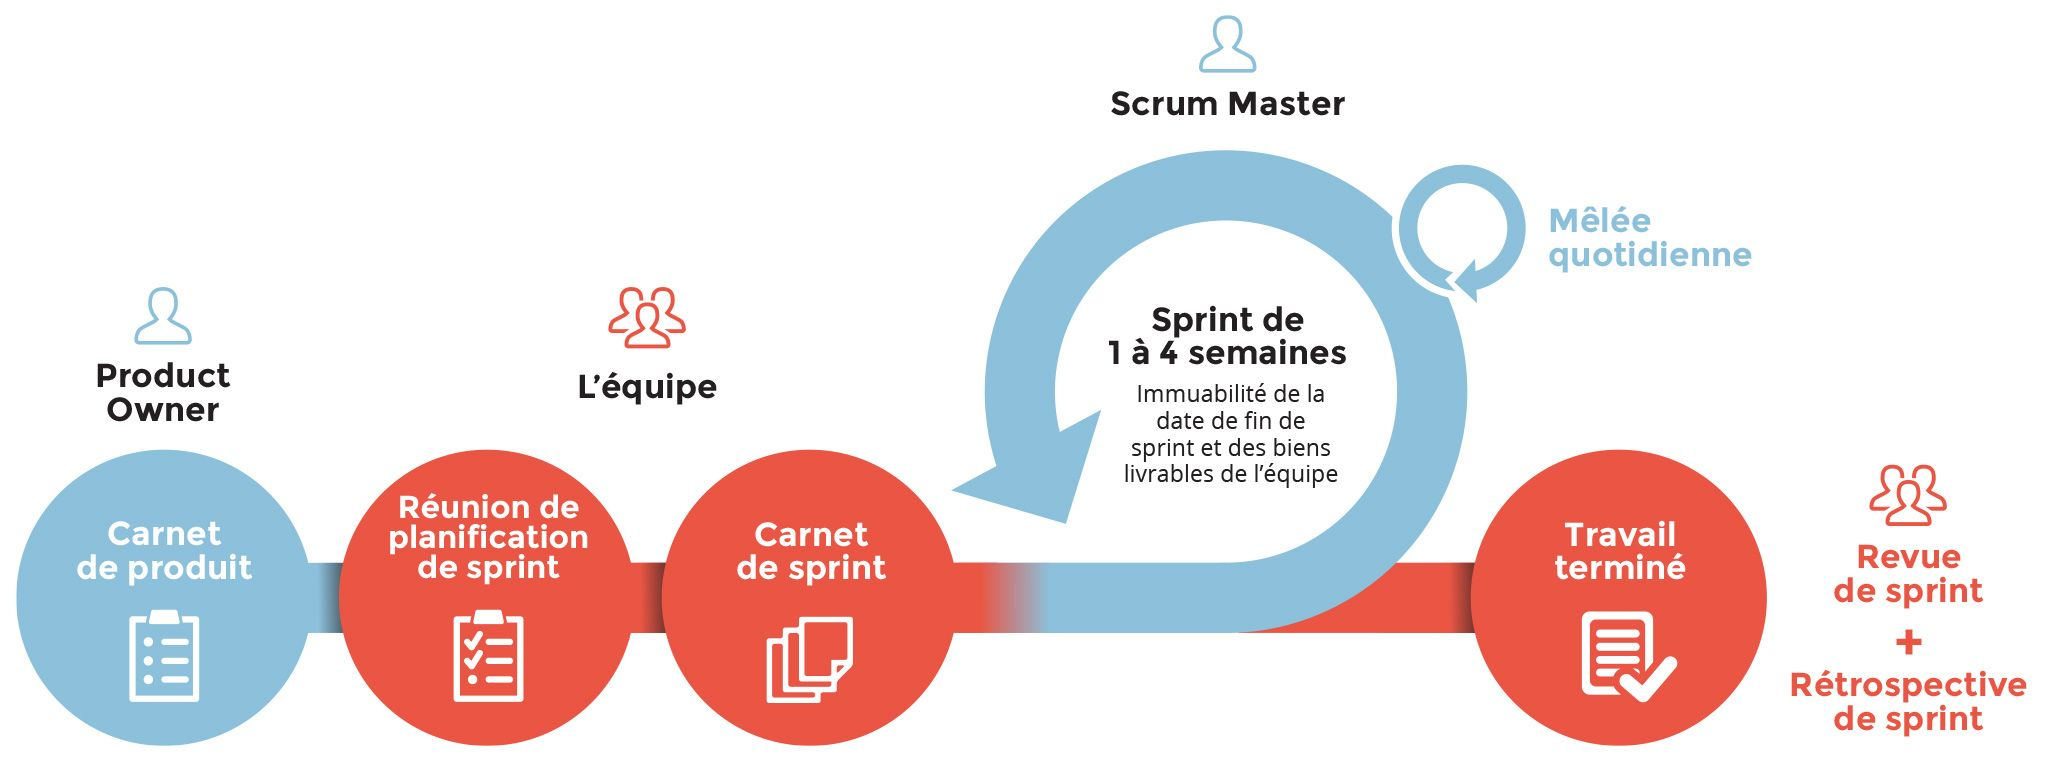
\includegraphics[width=1\linewidth]{img/scrum.jpeg}
    \caption{Schéma synthétique du processus \gls{scrum} (crédit \href{https://bubbleplan.net/blog/agile-scrum-gestion-projet/}{bubbleplan.net})}
\end{figure}

L'une de ses caractéristiques est la \emph{mêlée quotidienne}, couramment appelée \og \textit{daily} \fg pour \textit{daily scrum}, ou \og \textit{stand-up} \fg pour \textit{stand-up meeting}. C'est un point quotidien court -- d'où une réunion debout et non assis -- où chaque équipier rappelle ses tâches effectuées la veille, parle de ses points de blocage et termine par son programme de la journée.

Ces points permettent de débloquer les développeurs qui n'oseraient peut-être pas demander de l'aide autrement, par peur de déranger ou de passer pour incompétent. De plus, tout le monde peut suivre le projet dans sa globalité et mieux le comprendre grâce à cela. En plus de ces points, l'équipe se réunit à chaque début et fin de
\textit{sprint}\footnote{Période courte de 1 à 4 semaines pendant laquelle l'équipe doit terminer les objectifs décidés au préalable.}.

En début de période, l'on décide des tâches sur lesquelles l'effort sera concentré pour les semaines à venir. La planification se fait en équipe pour estimer au mieux la charge de travail nécessaire.

En fin de \textit{sprint}, on dresse le bilan des tâches accomplies et on en profite pour s'introspecter afin d'améliorer les méthodes de travail, les points de blocage de la période, la vie en équipe, etc.

Concernant le client, il voyait les avancées chaque semaine lors des points hebdomadaires, ainsi qu'en fin de \textit{sprint}.

Pour lui permettre de suivre le projet, nous lui avions donné un accès à une version de recette fonctionnelle du projet que nous mettions à jour à chaque fonctionnalité validée par les développeurs. Nous avions donc ses retours presque en temps réel.